\documentclass{article}

\usepackage{fancyhdr}
\usepackage{ragged2e}
\usepackage{graphicx}
\usepackage{caption}
\usepackage{geometry}
\usepackage{amsmath}
\usepackage{rotating}

\usepackage{listings}
\usepackage{color}

\definecolor{dkgreen}{rgb}{0,0.6,0}
\definecolor{gray}{rgb}{0.5,0.5,0.5}
\definecolor{mauve}{rgb}{0.58,0,0.82}

\lstset{frame=tb,
  language=Java,
  aboveskip=3mm,
  belowskip=3mm,
  showstringspaces=false,
  columns=flexible,
  basicstyle={\small\ttfamily},
  numbers=none,
  numberstyle=\tiny\color{gray},
  keywordstyle=\color{blue},
  commentstyle=\color{dkgreen},
  stringstyle=\color{mauve},
  breaklines=true,
  breakatwhitespace=true,
  tabsize=4
}

\setcounter{secnumdepth}{1}

\usepackage{chngcntr}
\counterwithin{figure}{section}

\renewcommand*{\thepage}{C\arabic{page}}

\pagestyle{fancy}
\lhead{ACME Robotics}
\chead{\#8367}
\rhead{\ifcontents Contents \else Week \thesection \fi}

\newif\ifcontents
\contentstrue

\makeatletter
\renewcommand{\@seccntformat}[1]{}
\makeatother

\begin{document}

\tableofcontents
\newpage
\contentsfalse
\clearpage \newpage \section{Week \thesection} 
\subsection{Business Goals}
\paragraph{B1: Draft and discuss this season's budget}
Draft budgets for the Software and Hardware Teams to determine fundraising goals and whether or not we can afford two competition robots.
\paragraph{B2: Complete fundraising and thank you letters}
Write two letters, one to last year's sponsors thanking them for supporting us, the other requesting funds from new and old sponsors.
\subsection{Hardware Goals}
\paragraph{H1: Build and test the glyph lifter at the 24-hour build}
Assemble the main lifter mechanism and lifter/grabber at the 24-hour build.
\paragraph{H2: Build and test the linear slide}
Assemble the basic slide and then customize it to the correct size and bulk.
\paragraph{H3: Build and test drive base}
The goal for the drive base is to create a platform on which the mechanisms can be mounted and tested. The requirements are that it has to have either two or four wheel drive, as well as a place to mount the phone, battery, and modules.
\subsection{Software Goals}
\paragraph{S1: Start learning new tools and software}
New members of the software team need to familiarize themselves with Java, Android Studio, and the FTC SDK.
\paragraph{S2: Test VuMark identification and Vuforia/OpenCV integration}
Get basic tracking and recognition of the pictographs (Vuforia VuMarks) working and convert Vuforia preview frames into Mats for OpenCV processing.	
\paragraph{S3: Explore options for cipher cube pattern assistance}
Explore the possibility of using software to intelligently choose what color glyph to pick up and where to put it, to make a pattern, as well as keep our options open.
\paragraph{S4: Brainstorm potential uses of software in the game}
Brainstorm potential uses for software control in both autonomous robot operation and driver assistance in teleop.
\newpage
\subsection{B1: Draft and discuss this season's budget}

In preparation for the coming season, Kellen and Ryan devised two budgets for the Hardware and Software Teams respectively. For the Hardware team, the budget consisted primarily of planned purchases of Tetrix parts, tools, and motors/servos. For the Software Team, the budget was mainly concerned with buying new phones and migrating to the new REV control system. As a group, we tallied the estimated expenses and profits for team membership fees and determined our fundraising goals for this year based on travel/registration costs from previous seasons, which was six thousand dollars. We also decided that we had enough money and resources to build two competition robots this season. See Appendix A in the Business Notebook for more details.

\subsection{B2: Complete fundraising and thank you letters}

This week Emma and Clara worked on writing two letters to our sponsors.  The first was a thank you letter, written to last year's sponsors thanking them for all of their generous support during last season. The second was the fundraising letter sent to various potential and current sponsors asking for donations for the coming season. The letters can be seen in Appendix B of the Business Notebook. The letter included our new system of donations, which uses tiers to provide the sponsor with varied levels of publicity on our website and social media. These tiers can provide the sponsor with anything from a shout out on social media to a private presentation of the robot.  These tiers are to provide the donor with a clear description of what they will receive if they fund us. The letters will be sent out to local businesses and companies. 
\subsection{H1: Build and test the glyph lifter at the 24-hour build}

At the 24 hour build, the Hardware Team's goal was to build a working lifter/grabber on a functional drive base. In the beginning, we drew sketches of potential lifter designs. Then, once we had a few ideas on a lifter mechanism shown in figure \ref{fig:brainstorm}, we started to test different lifters that we had sketched out. 
\begin{figure}[h]
    \centering
    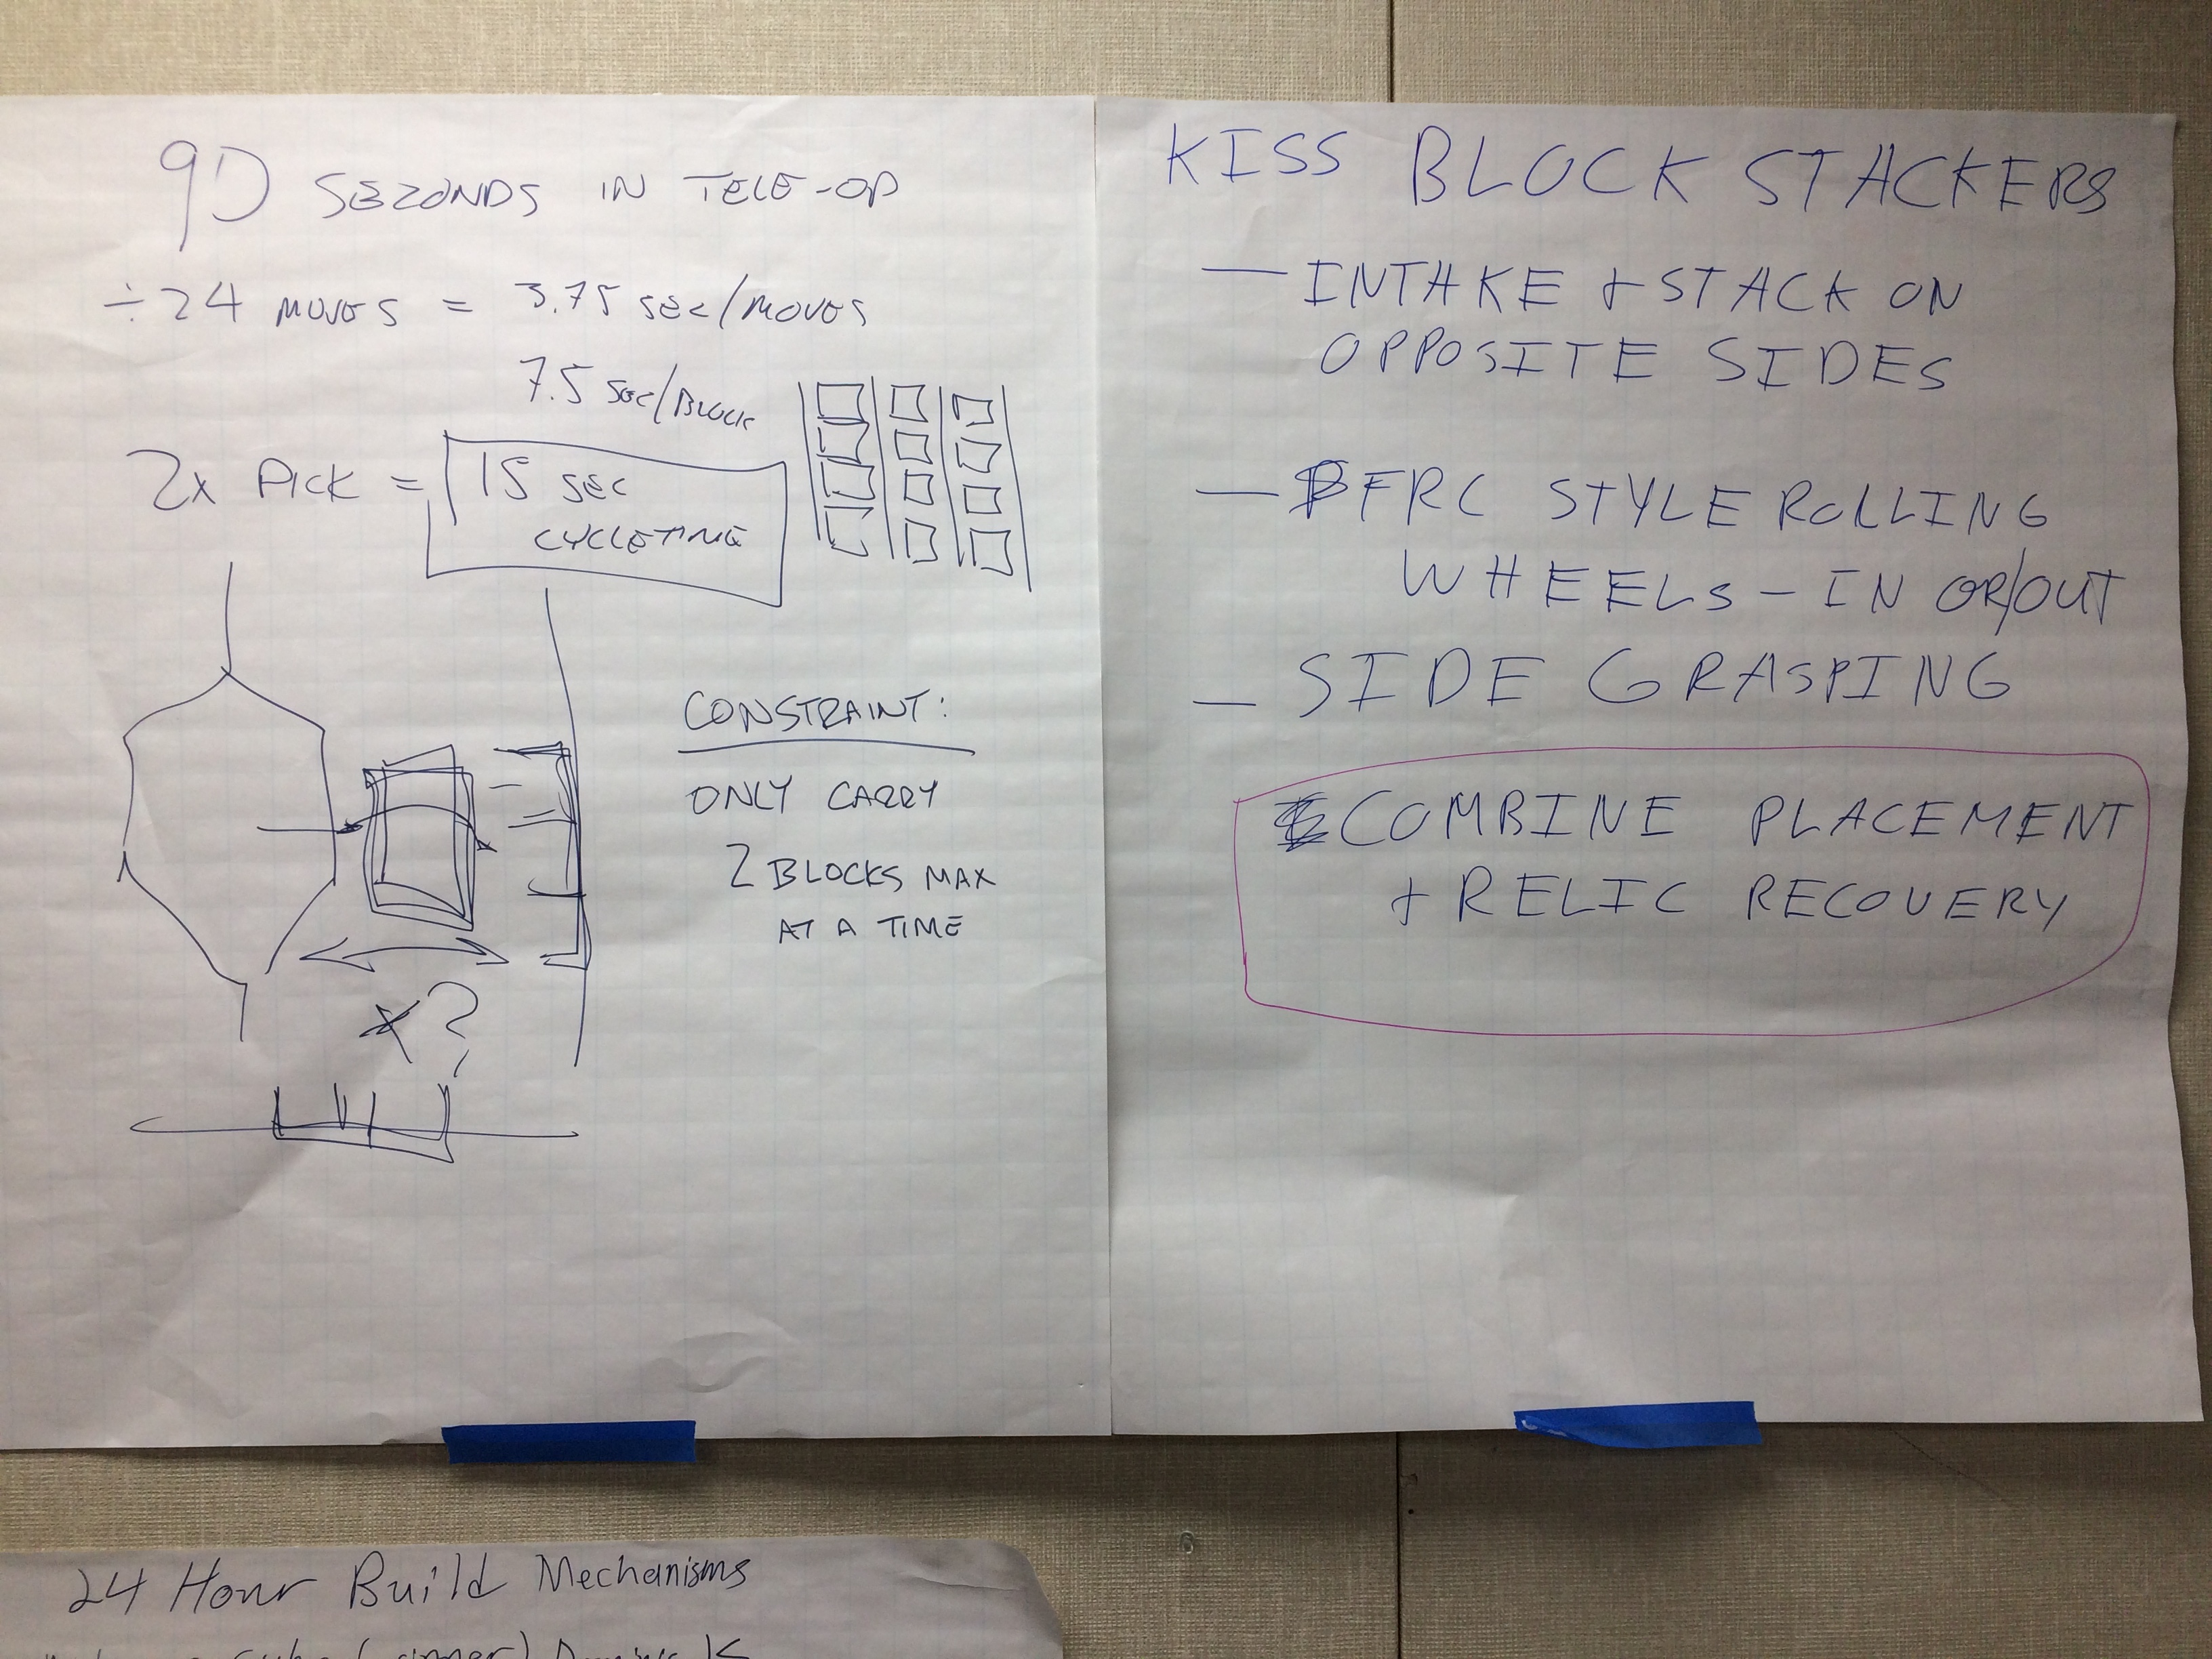
\includegraphics[width=.8\textwidth]{01/images/brainstorm.jpg}
    \caption{brainstormting}
    \label{fig:brainstorm}
\end{figure}
After testing the different ideas, our final decision was a parallel lift, driven on one side. We then started the building and assembly of the grabber. This took us a few hours to complete and put onto the drive base. We came across a few struggles, such as parts not cooperating, broken parts, and flaws in the design. This included the arm not being rigid enough, which was resolved by putting cross braces across the arm. The gears powering the arm were skipping, due to misalignment, but this was solved by the addition of shims and Zip Ties. In the end, we had a fully functional lifter, that can be seen in figure \ref{fig:robot}. We tested this mechanism, and it worked for the most part, other than us having to come up with a way to grip the glyphs and lift them up. 
\begin{figure}[h]
    \centering
    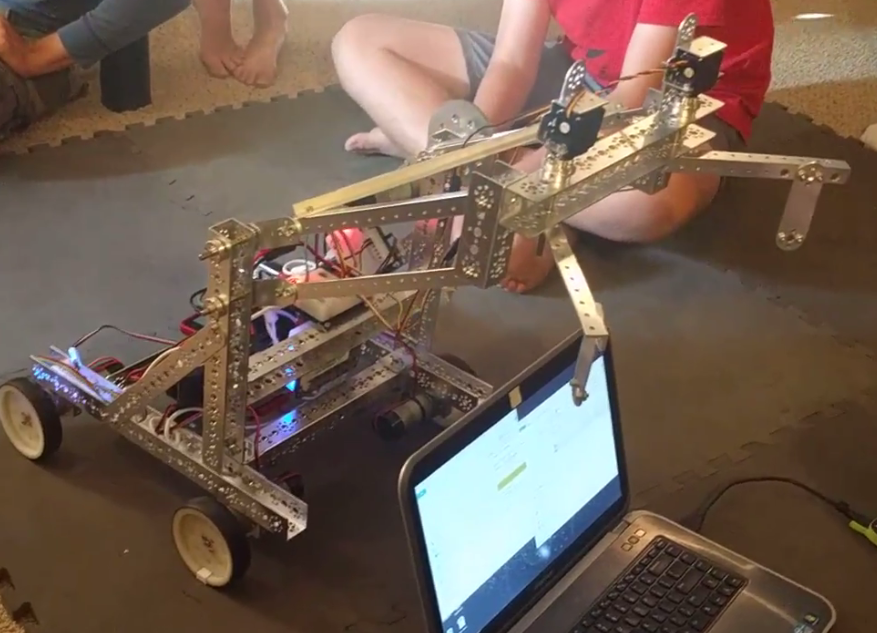
\includegraphics[width=.6\textwidth]{01/images/robot.png}
    \caption{robot}
    \label{fig:robot}
\end{figure}

\subsection{H2: Build and test the linear slide}

At the 24-hour build,  Ben was assigned the task of building the linear slide for the relic. He watched the REV linear motion kit how-to video and assembled the slide without difficulty. Then, our mentor Mike and Ben drew some sketches of our visions for the linear slide and how it was going to work. He decided on a design that allowed the slide to fit into the sizing cube and not take up a lot of bulk. Next, he put the metal stock into a vise and hack sawed them into 16 inch lengths. Finally, he assembled the slide according to the drawings. Also, he had to add WD-40 to make the mechanism slide smoother. He also made some sketches of the slide before he started cutting things. Figure \ref{fig:sketch} shows the sketch that Ben and Mike made before they cut the extrusion.
\begin{figure}[h]
    \centering
    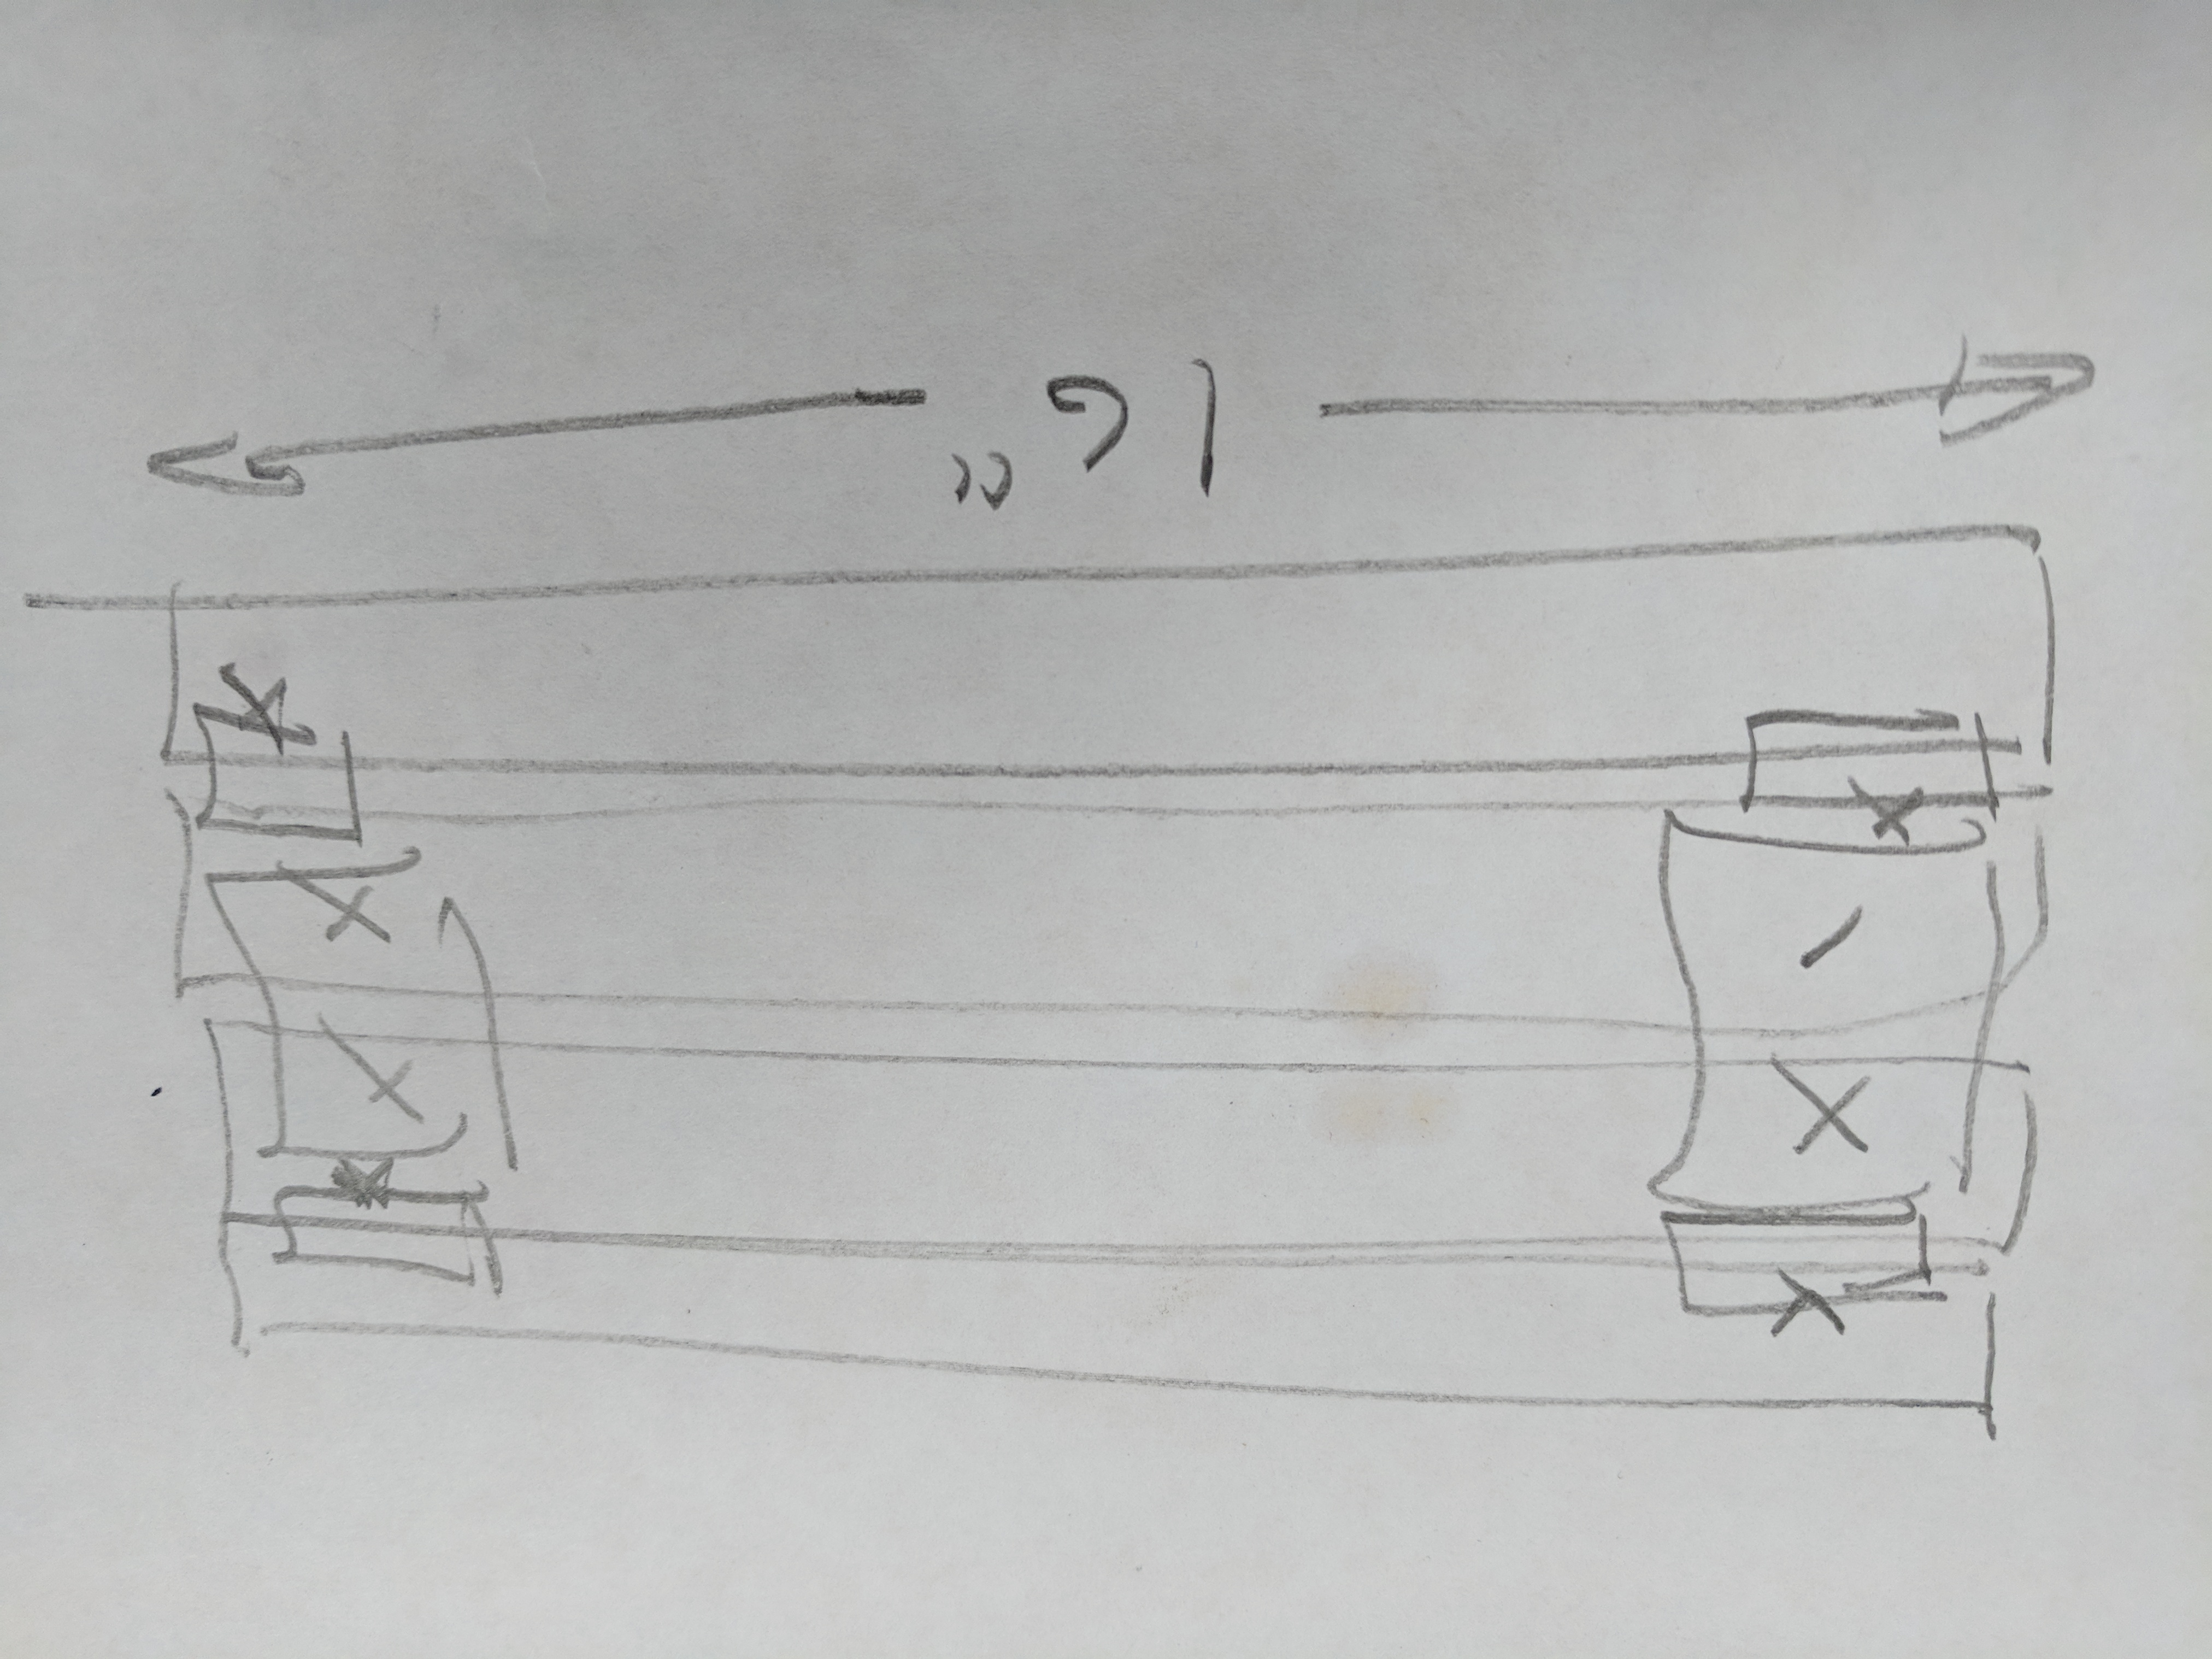
\includegraphics[width=.6\textwidth]{01/images/Sketch2.jpg}
    \caption{sketch}
    \label{fig:sketch}
\end{figure}

\subsection{H3: Build and test drive base}

For the 24 hour build, we needed a drive base to attach whatever mechanisms we made to in order to test them properly. We had a test base already built to test the REV module, with phone and battery mounts as well as four motors and wheels. We decided to modify this base instead of building a new one around the mechanism because it was less time consuming and worked just as well. In order for the mechanism to work, we replaced the small tetrix wheels on the base with larger ones, moved the motors inwards, away from the corners, and moved the position of the modules. In the end, the drive base functioned perfectly and allowed us to test all the modules we wanted.
\subsection{S1: Start learning new tools and software}

Emma and Clara completed a Code Academy Tutorial to learn the basics of Java, the language that the FTC app is programmed in. Then, inheritance was worked on because it is a major concept within the FTC SDK. Knowing how to do this will make understanding the code of the robot easier. Afterwards, a PowerPoint was reviewed that showed how to use Android Studio to practice coding.  The PowerPoint also gave examples and explained various function meanings in-depth. A TeleOp program was then written afterwards. Emma and Clara then set up and worked on the Modern Robotics training modules to help learn how to use sensors. It is crucial to know how to do this because sensors will need to be used for the new tasks of the robot. TeleOp code was looked at as well, followed by a series of videos for more in depth information.

\subsection{S2: Test VuMark identification and Vuforia/OpenCV integration}

By copying and slightly modifying the Concept VuMark Identification sample in the SDK, Ryan was able to quickly get VuMark identification working. The Opmode was successfully able to track the VuMarks and report both the autonomous bonus cryptobox column and the location of the VuMark. After that, Ryan researched how to convert Vuforia ClosableFrames to OpenCV Mats. Using some of the code from last year, he was able to extract grayscale images. His first attempts to get RGB frames were frustratingly unsuccessful until he figured out that the command to generate RGB frames had to be issued after the rest of the preview had initialized. Once this was figured out, the images were all loaded properly and ready for custom processing. The software team has decided to use OpenCV to try to ascertain the position of the jewels in autonomous; this is Ryan's next goal. A screenshot of VuMark identification is shown in figure \ref{fig:vumark}.
\begin{figure}[h]
    \centering
    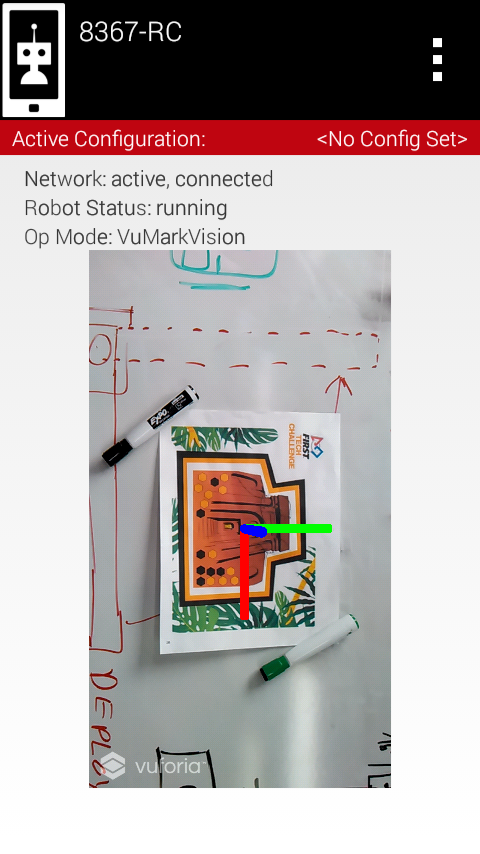
\includegraphics[width=.6\textwidth,height=3in,keepaspectratio]{01/images/vumark.png}
    \caption{Vuforia VuMark identification}
    \label{fig:vumark}
\end{figure}

\subsection{S3: Explore options for cipher cube pattern assistance}

In order to place the glyphs in patterns to correctly make the ciphers, scoring points, and allowing us to begin scoring a relic earlier, the process of choosing a color and where to place it had to be streamlined. Scenarios where it is only easy to pick up one color but there is nowhere for it to go drastically reduce the efficiency of glyph placement by forcing the robot to sort through the glyph pile. When the robot is able to choose between the two colors, the choice that maximizes future flexibility should be selected. The first idea was to use something similar to a minimax search algorithm, used for game playing algorithms. All the possible end states of the game are assigned a value, representing how desirable they are for one of the players. Then, working backward, it is assumed that the first player will always make the move that will maximize that value, and the other player, on their turn, will make the move that minimizes that value, an example of this is shown in figure \ref{fig:minimax}.
\begin{figure}[h]
    \centering
    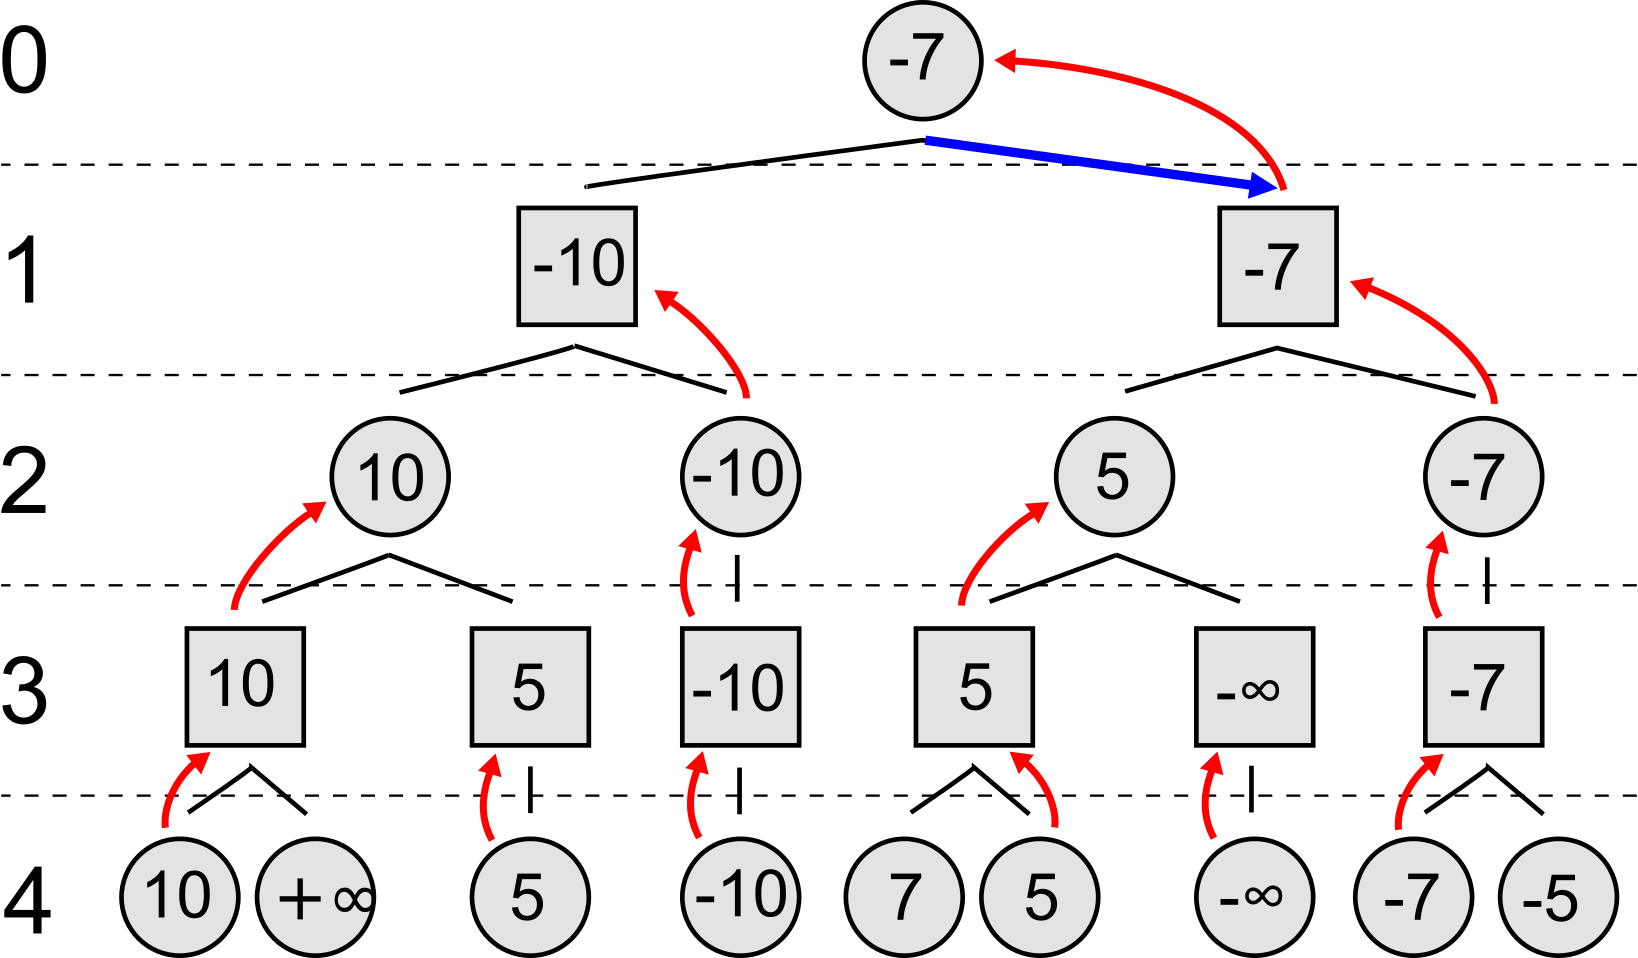
\includegraphics[width=.6\textwidth]{01/images/minimax.png}
    \caption{minimax algorithm}
    \label{fig:minimax}
\end{figure}
A similar algorithm could be applied to this problem, determining the flexibility afforded the robot at each possible state of the cipher cube, and then working backward, maximizing that flexibility at every decision, to decide what move to make to keep the most flexibility. Using this concept, the first attempt laid out all the possible cipher states in a tree. At the top is the initial configuration of the cipher, all empty. The children of each node are determined by enumerating all possible additions of a single cube, and then eliminating all states that cannot be made into a correct cipher. Each node was assigned a value of 0 if it was constraining, meaning that there is only one color of cube that could be added to the current state. To determine how desirable a node was the average value of all its children was taken. A higher number meant that, if that node was reached, the remaining cubes to be taken in and placed would be more flexible. This was a good representation of the flexibility of a state, but took a long time to run. With 12 moves, and 6 choices at each move (2 colors and 3 columns), there were $6^12$, or $2,176,782,336$ possible configurations of the cipher. One option to address this is to only search so deep into the tree. This greatly reduces the computational intensity. Another option is to come up with a function that estimates the desirability of a state.


\subsection{S4: Brainstorm potential uses of software in the game}

The software team analyzed different opportunities to use software to enhance the robot's capabilities in autonomous and teleop. In particular, we discussed methods for jewel identification and cryptobox alignment.	The software team brainstormed how effective software could be used in Relic Recovery to enhance the robot's performance. In autonomous, the two primary tasks are knocking the proper jewel and scoring glyphs in the cryptobox. For jewel identification, they discussed two potential methods, one using color sensors and another using vision. The color sensor initially seemed promising and hopefully simpler, but early tests revealed that the sensor had to be quite close to the jewel to get a reliable reading and not be pointing into one of the holes. In the end, the success of this method would largely depend on the orientation of the jewel and the consistency of the jewel manipulator/initial robot placement. The vision-based approach helps solve both these issues with the cost of some added complexity. Furthermore, the camera will already be pointed in the direction of the jewel stand to read the pictograph. After weighing the advantages and disadvantages of both approaches, the software team decided to pursue OpenCV-based color detection for jewel identification. For glyph scoring, the primary difficulty seems to be properly aligning with the cryptobox. Although dead reckoning from our starting position could work, it isn't very robust and errors accumulate quickly (especially if the robot makes multiple scoring runs in autonomous). Furthermore, it would be helpful to have similar alignment functionality in teleop to assist the drivers and score glyphs more quickly. Unfortunately, the pictographs aren't optimally placed for cryptobox alignment; there are none nearby the side/auxiliary box and they become occluded as the robot approaches the cryptobox. The only solution the team came up with was again using vision to detect the cryptobox and use its positioning in the image and the robot orientation from the IMU to align. Although rather complex and potentially unstable, this seems like the only solution that satisfies the requirements.
\clearpage \newpage \section{Week \thesection} 
\subsection{Hardware Goals}
\paragraph{H1: Make a longer and working linear slide for the relic gripper}
Reassemble the original slide and make it a single to make it longer and function better.
\paragraph{H2: Prepare Inventor files for the Glyph lifter}
Download files from GrabCAD and find files on hard drive that are necessary to create the Glyph lifter to start designing it.
\paragraph{H3: Research the most efficient type of drivetrain}
Research successful drivetrains that other teams have used to win, and decide on a drivetrain to construct for this season.
\subsection{Software Goals}
\paragraph{S1: Write code to identify the position of the jewels using vision}
Use OpenCV and basic image processing to reliably determine the state of the jewels during autonomous.
\paragraph{S2: Setup version control and task tracking and explain the general software workflow to new members}
Setup a new repo on GitHub for this season, with the task tracker we will be using, Jira, and continuous integration. Explain the software workflow with Git and Jira to the new software members.
\paragraph{S3: Write dead reckoning code for localizing the robot.}
Use data from only the encoders and gyro to determine the position of the robot on the field, for executing path and placing glyphs.
\newpage
\subsection{H1: Make a longer and working linear slide for the relic gripper}

Ben used the oil to oil the linear slide and noticed that nothing was happening at all. He was helped by Shawn and they found out why the slide wasn't sliding the best. The screws on the sliding plastic piece couldn't be tightened all the way or else the slide wouldn't slide correctly. This happened because the extruded aluminum the slide is made of was being bitten into by the tight screw so it didn't slide smoothly at all. It took a great deal more of force to move the slide than it should have. This was easily solved by un-tightening the screws and making them kind of tight, but not enough to engage the aluminum. This they did and found out the secret of the slide. This took most of the meeting but they still had some time before the end, so they started on the claw to grab the relic. Figure \ref{fig:claw} shows the finished claw gripping the relic.
\begin{figure}[h]
    \centering
    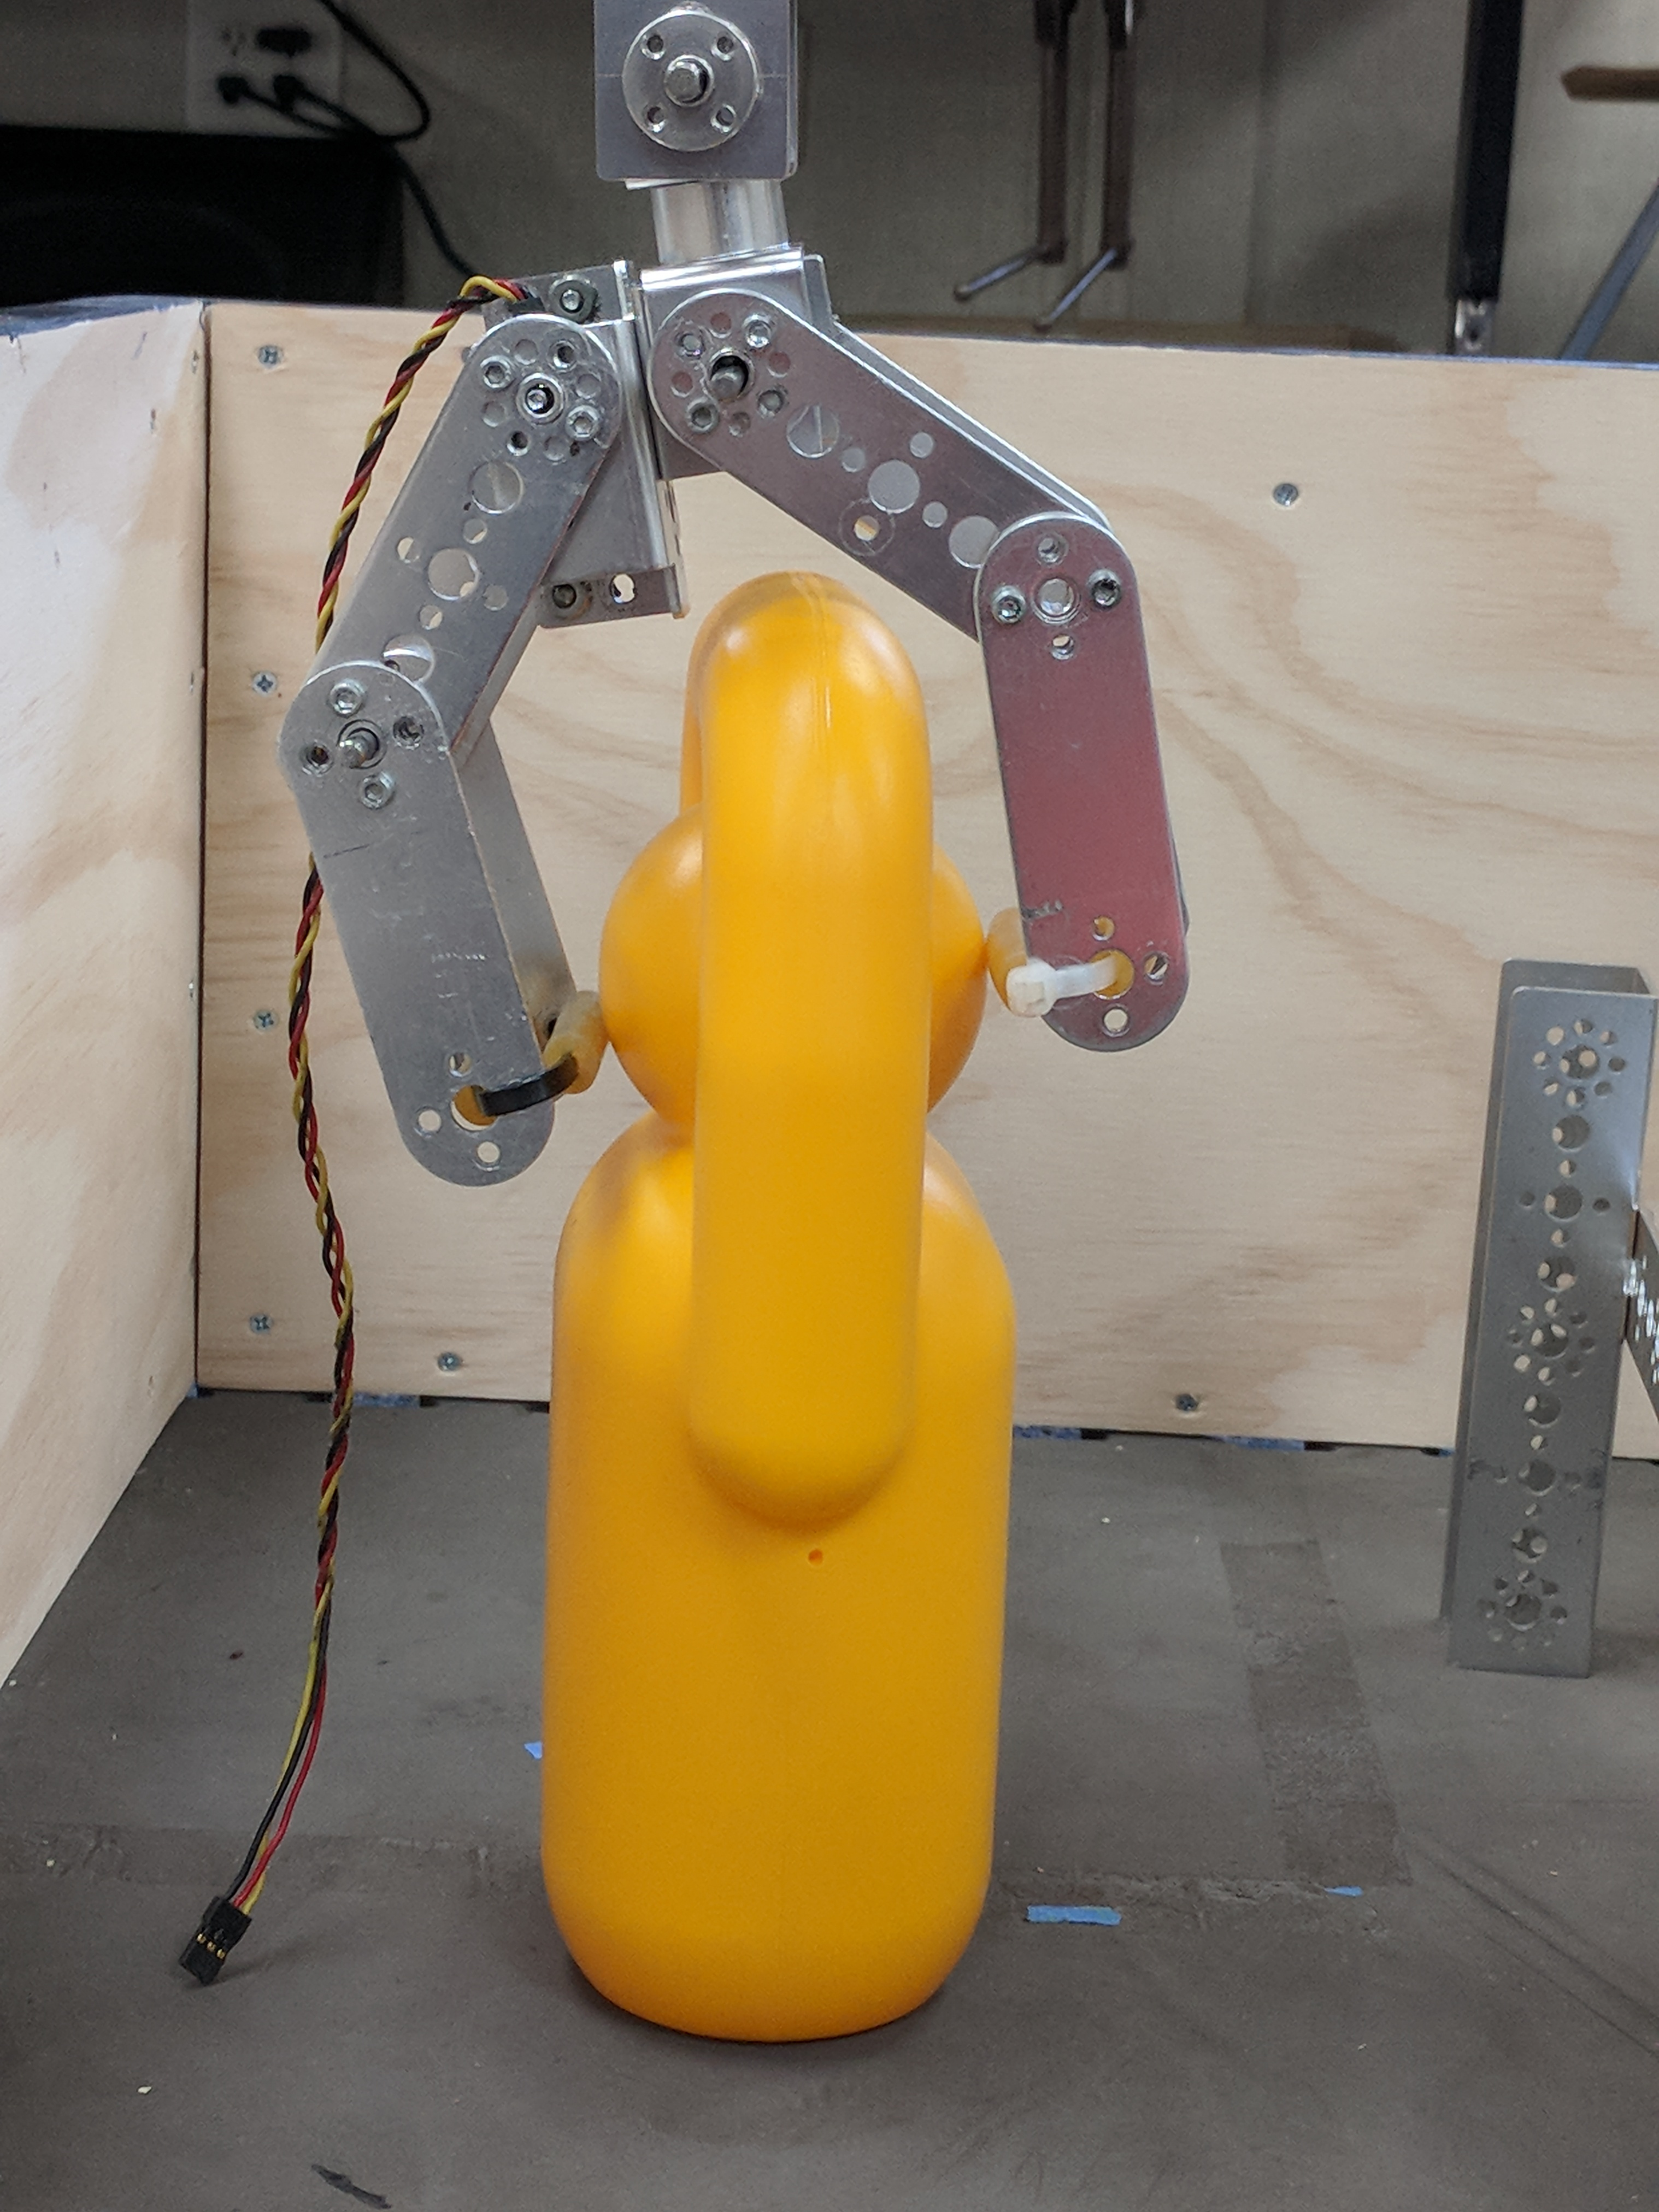
\includegraphics[width=.6\textwidth]{02/images/clawgrippingrelic.jpg}
    \caption{claw}
    \label{fig:claw}
\end{figure}

\subsection{H2: Prepare Inventor files for the Glyph lifter}

John went onto GrabCAD and downloaded all parts necessary to create the Glyph lifter. John also went through the files from last year to find all useful parts for the lifter. Afterward he started the rough design of the lifter. We decided to use a lead screw for raising and lowering the mechanism because it would take up less space and be able to raise a large load. The initial design is shown in figure \ref{fig:leadscrew}. Some small changes were made from the original idea including the secondary lifting mechanism that would be necessary for the lifter to reach the fourth row, and the mounting points for the glyph holder.
\begin{figure}[h]
    \centering
    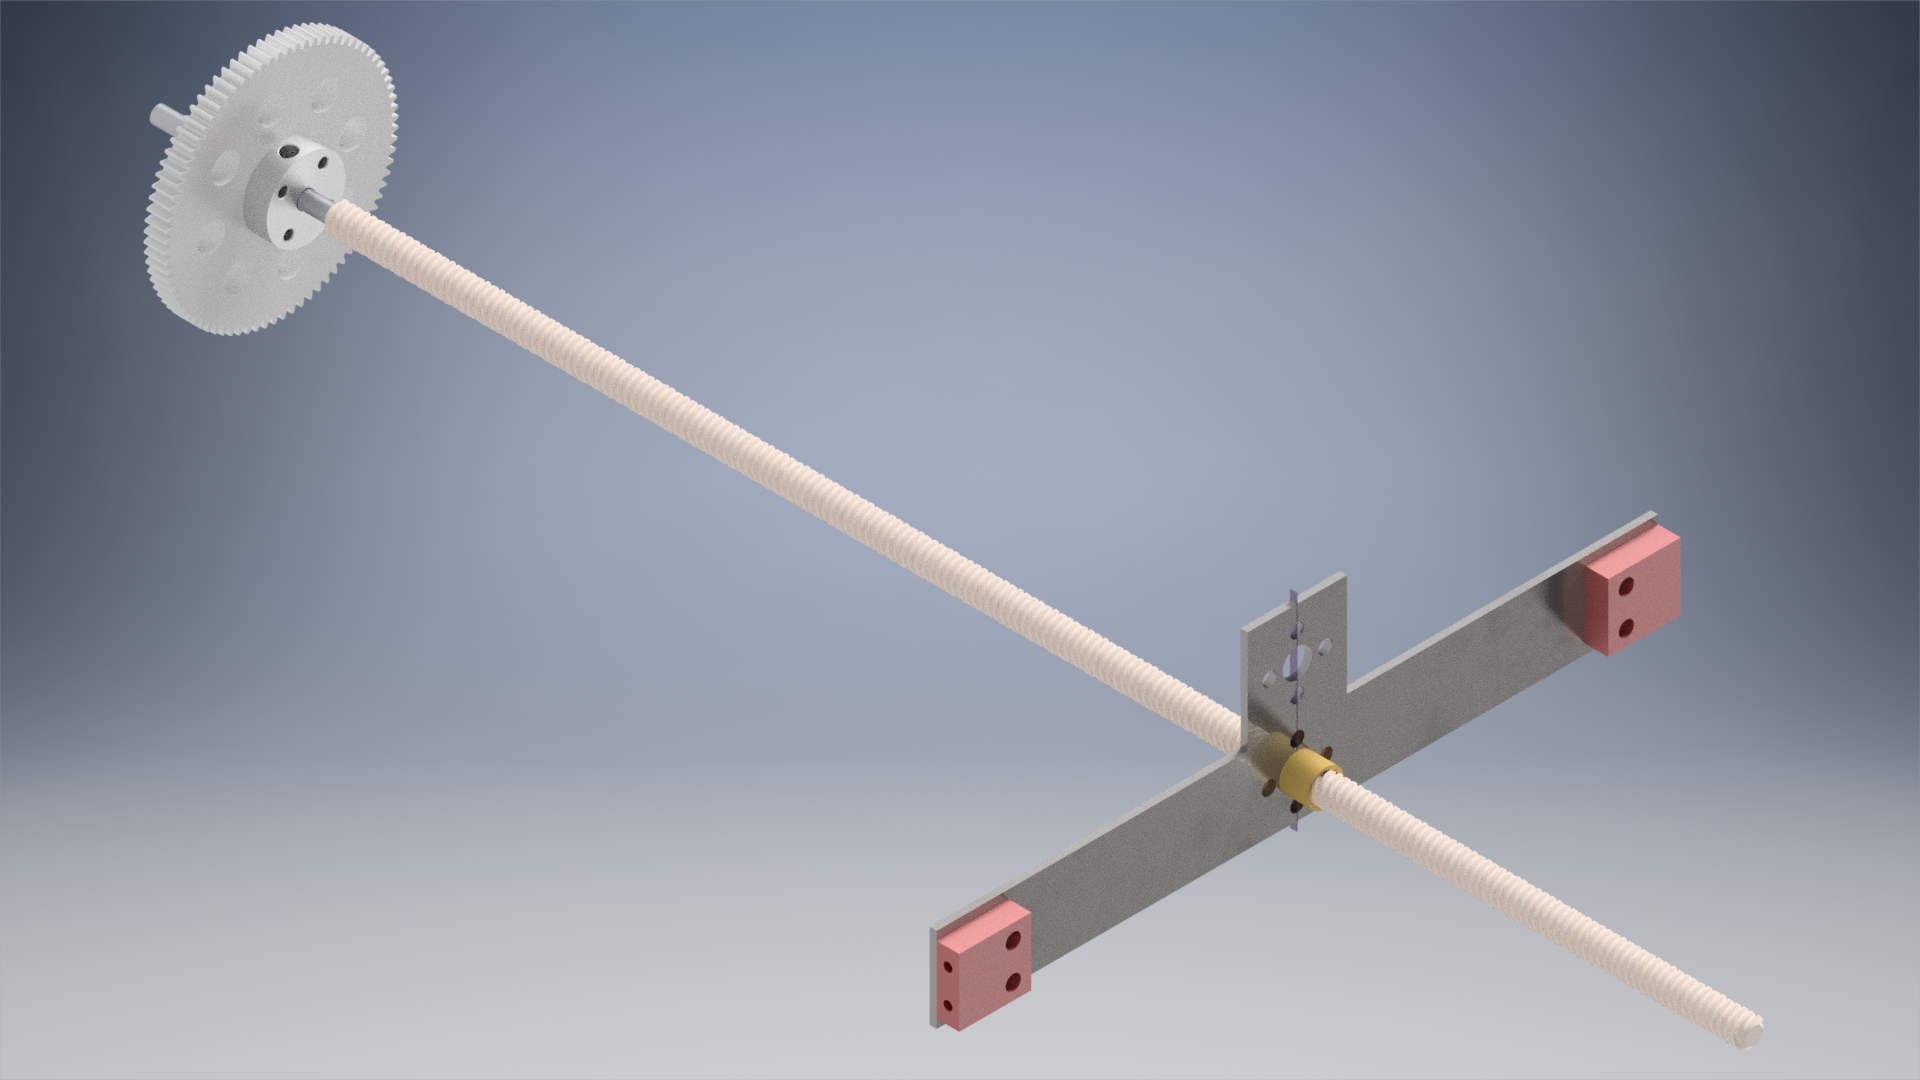
\includegraphics[width=.6\textwidth]{02/images/leadscrew.png}
    \caption{a lead screw}
    \label{fig:leadscrew}
\end{figure}

\subsection{H3: Research the most efficient type of drivetrain}

Oren and Dominick did a ton of research on other teams' successful drivetrains and decided on a direction to take for the drivetrain division. They narrowed the choices down to a mecanum drive, and three variations of 6-wheeled tank drive, 6 wheel direct drive, 6 wheel with drop center, and 6 wheel with omni front and back wheels. They were able to elimane swerve drives early due to their complexity, and an omni drive because it was less reliable and provided no advantages over mecanum. The options, as well as their pros and cons, are shown in figure \ref{fig:options}. They decided that a mecanum drive would be best, because it could provide the key maneuverability necessary for aligning with the cryptobox, and there is no need for the high traction necessary in games with more defensive play. The next step for the drivetrain team is to decide how to drive each mecanum wheel.
\begin{figure}[h]
    \centering
    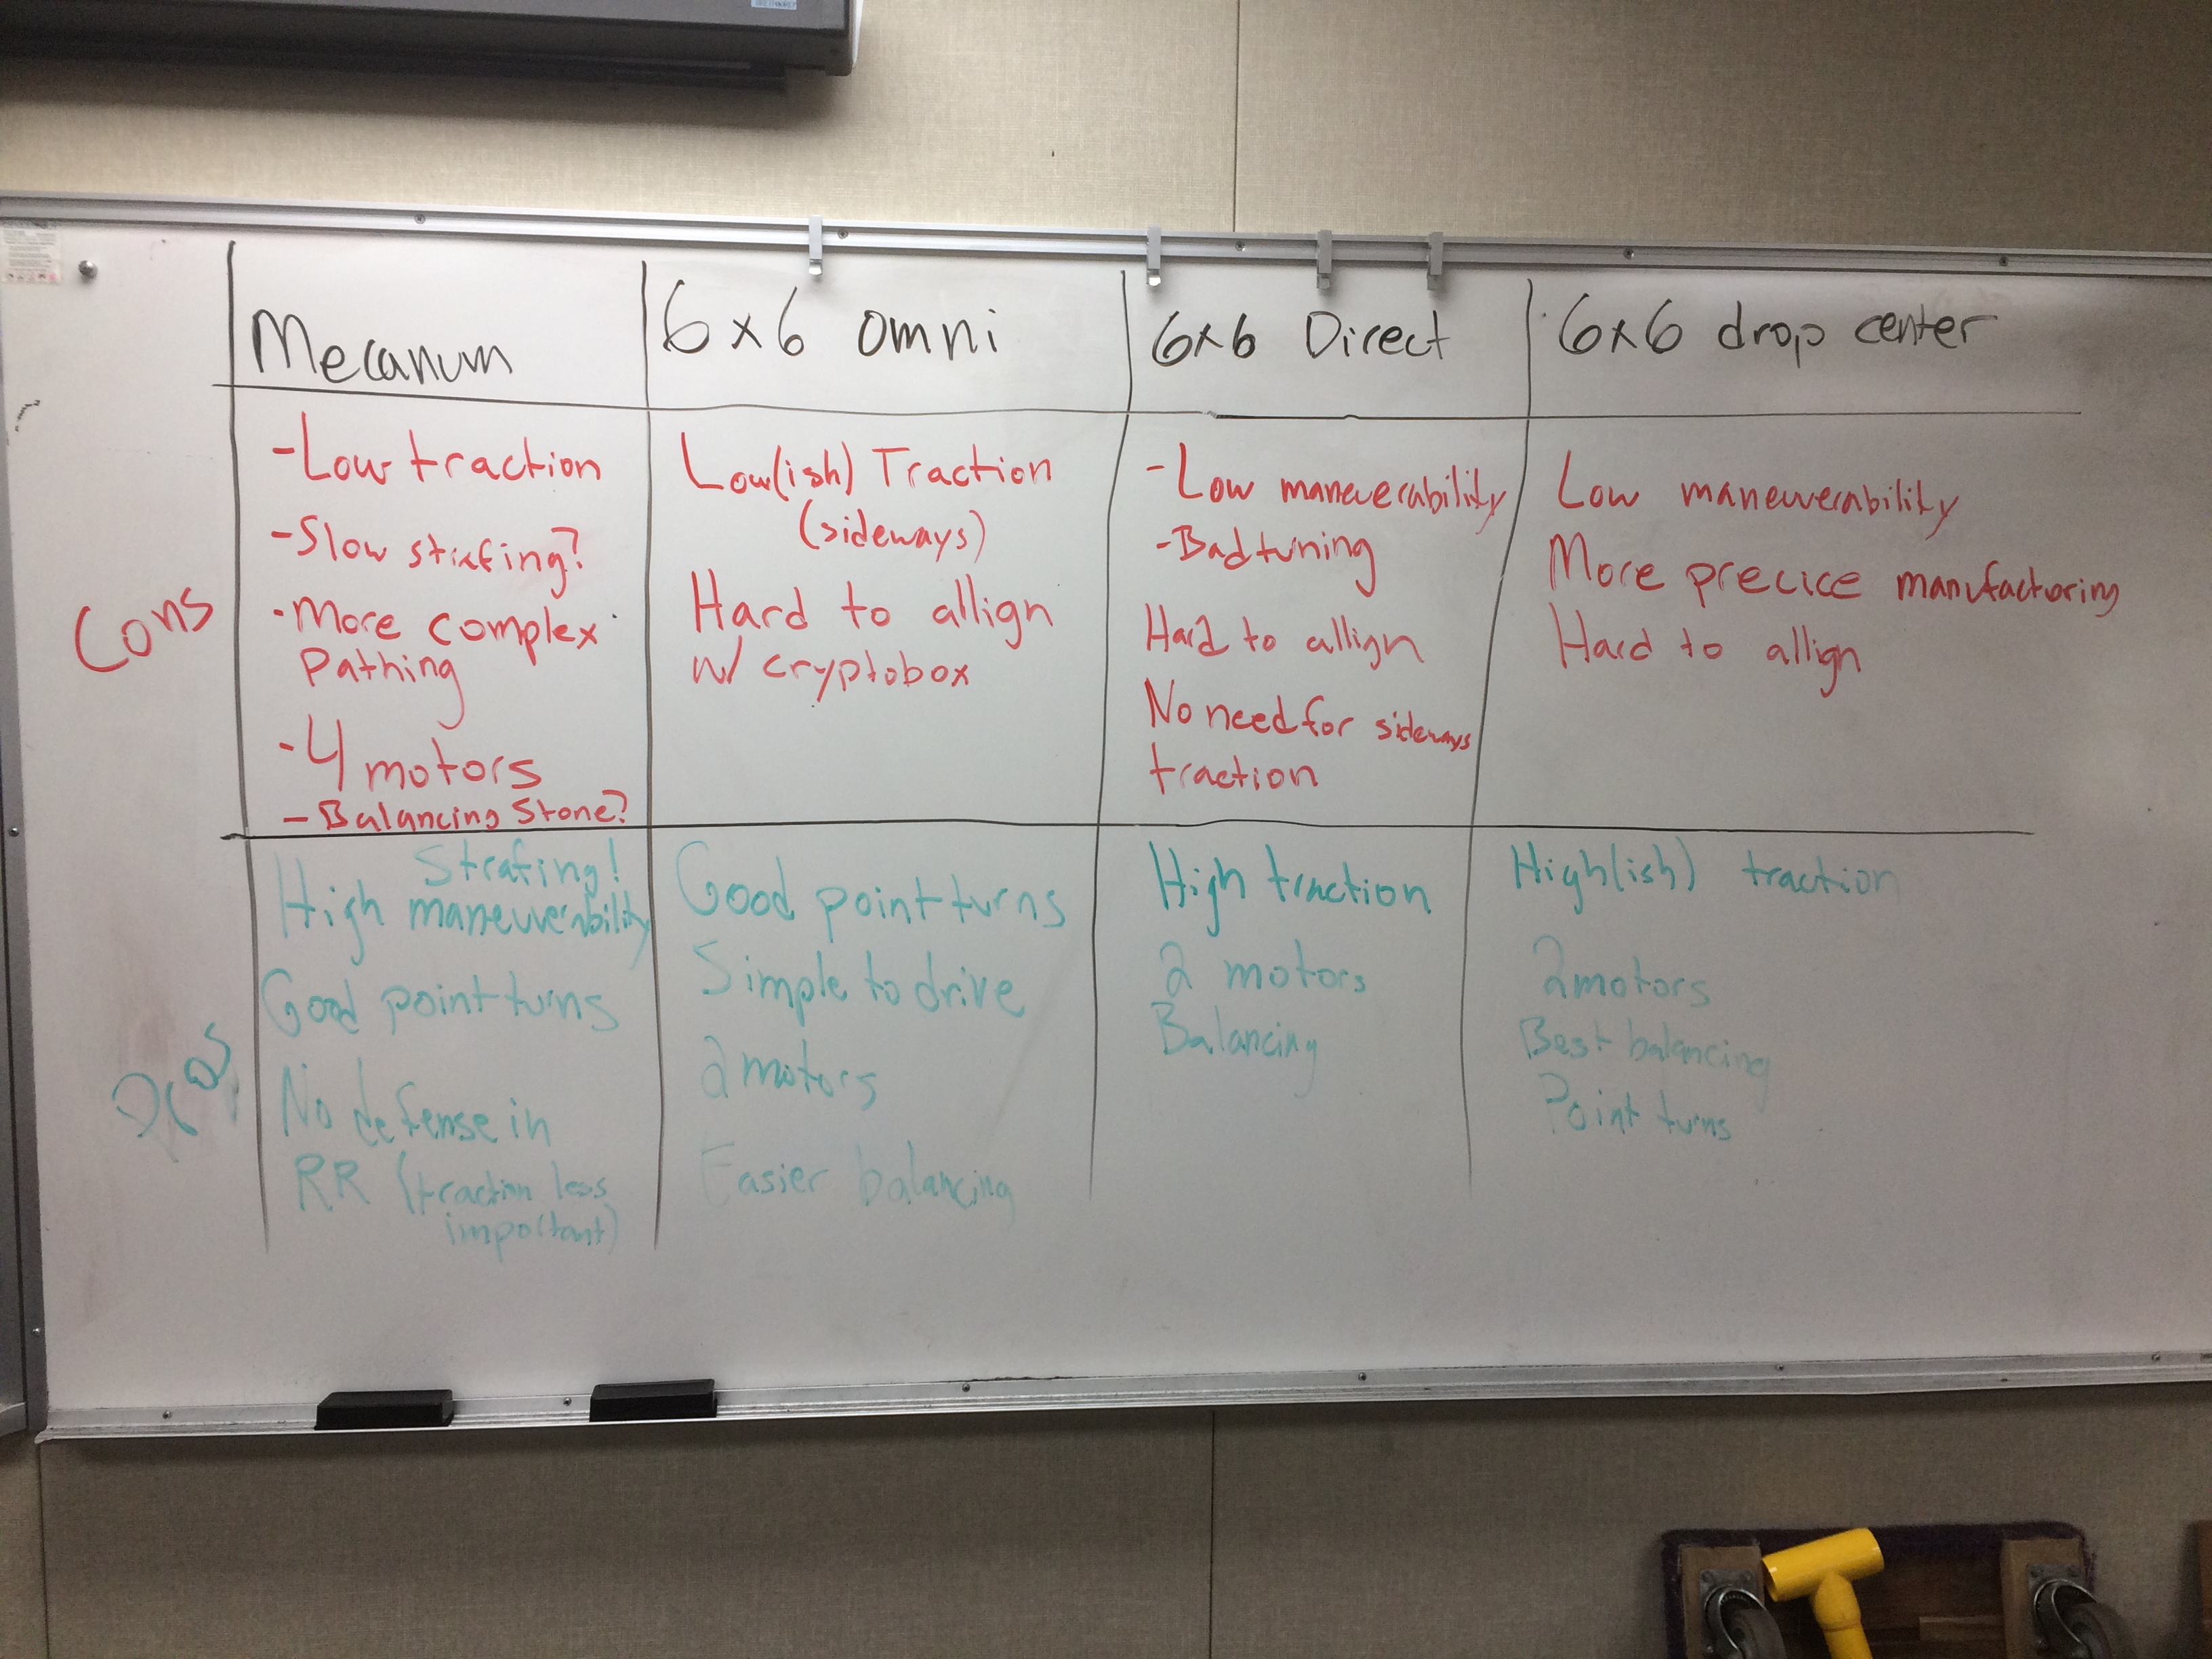
\includegraphics[width=.6\textwidth]{02/images/options.jpg}
    \caption{some of the options}
    \label{fig:options}
\end{figure}
\subsection{S1: Write code to identify the position of the jewels using vision}

Ryan worked on a basic jewel vision system. Although the actual algorithm/image processing is simple, there's a lot of ``glue'' code necessary to get vision working properly. During the 24-hour build, Ryan was able to download and add OpenCV to the Android project, and, after some frustrating debugging, he was able to convert Vuforia preview frames into OpenCV mats. Ryan used this code to get OpenCV images from the Vuforia preview. Specific regions from the jewel were then cropped out of the image and used to compute the average RGB color. Here's the code for computing the red/blue color ratios:
\begin{lstlisting}[language=Java]
Mat leftJewelCropped = rgb.submat(leftJewelRect);
Mat rightJewelCropped = rgb.submat(rightJewelRect);

Scalar leftJewelTotalColor = Core.sumElems(leftJewelCropped);
Scalar rightJewelTotalColor = Core.sumElems(rightJewelCropped);

leftBlue = leftJewelTotalColor.val[0];
leftRed = leftJewelTotalColor.val[2];
rightBlue = rightJewelTotalColor.val[0];
rightRed = rightJewelTotalColor.val[2];

double leftTotal = leftBlue + leftRed;
double rightTotal = rightBlue + rightRed;

if (leftTotal == 0) {
    leftBlue = 0;
    leftRed = 0;
} else {
    leftBlue /= leftTotal;
    leftRed /= leftTotal;
}

if (rightTotal == 0) {
    rightBlue = 0;
    rightRed = 0;
} else {
    rightBlue /= rightTotal;
    rightRed /= rightTotal;
}
\end{lstlisting}

This can then be easily converted into a binary red/blue or blue/red jewel configuration output. The next bit of glue code involves superimposing an overlay on top of the preview and drawing the jewel rects with the appropriate color. This was actually the most difficult part of the whole thing; it took many tries to get the canvas transforms working properly. However, in the end, everything went together nicely and was able to accurately assess the jewel colors. Michael, Kelly, and Ryan also tested it briefly in different lighting conditions and it worked flawlessly. Figure \ref{fig:vision} shows a screenshot of the end result.
\begin{figure}[h]
    \centering
    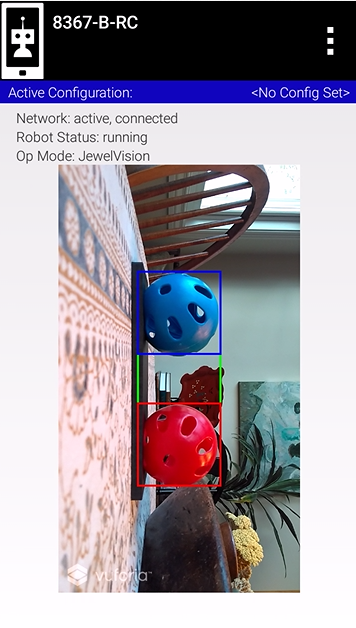
\includegraphics[width=.6\textwidth,height=3in,keepaspectratio]{02/images/jewelvision.PNG}
    \caption{Caption}
    \label{fig:vision}
\end{figure}

\subsection{S2: Setup version control and task tracking and explain the general software workflow to new members}

Ryan setup a new Android Studio project with the SDK in a separate directory. He also copied some of the necessary files from previous seasons and added CI. Michael also introduced Jira to the team. The team decided that some kind of issue tracking functionality would help organize the software tasks, especially between multiple people. They also decided to have a more well-defined, systematic procedure for integrating changes. For the most part, new features will be created in separate branches corresponding to issues in Jira. Once the changes are ready, a pull request will be created and the code will be reviewed before finally be merged into the master branch. Overall, this workflow keeps the master branch clean and operational (in theory) and the whole repo structurally better. 

\subsection{S3: Write dead reckoning code for localizing the robot.}

Kelly worked on dead reckoning code. When location cannot be determined by vison, either Vuforia or some sort of cryptobox detection, the position of the robot can be estimated by measuring movements using internal sensors (encoders on the drive motors and the gyro), and keeping track of the robots movement from the last known position. When working with a tank drive style drive base, it is best to assume that each incremental movement that is being measured is in an arc, rather than a straight line, in order to reduce error. The average displacement of all drive motor encoders is used to determine the distance the robot has travelled, and then the angular displacement is measured from the gyro, this is shown in figure \ref{fig:twist}. When the arc length and angle are known, the radius and chord length of the arc can be calculated, using $$r=\frac{l_{arc}}{\theta}$$ $$l_{chord} = r \sqrt{2(1-\cos{\theta})}$$. The motion of the robot can then be represented in polar coordinates, theta is equal to the final heading of the robot, and r is equal to the chord length. It is then easy to convert to cartesian coordinates and find the updated position of the robot.
\begin{figure}[h]
    \centering
    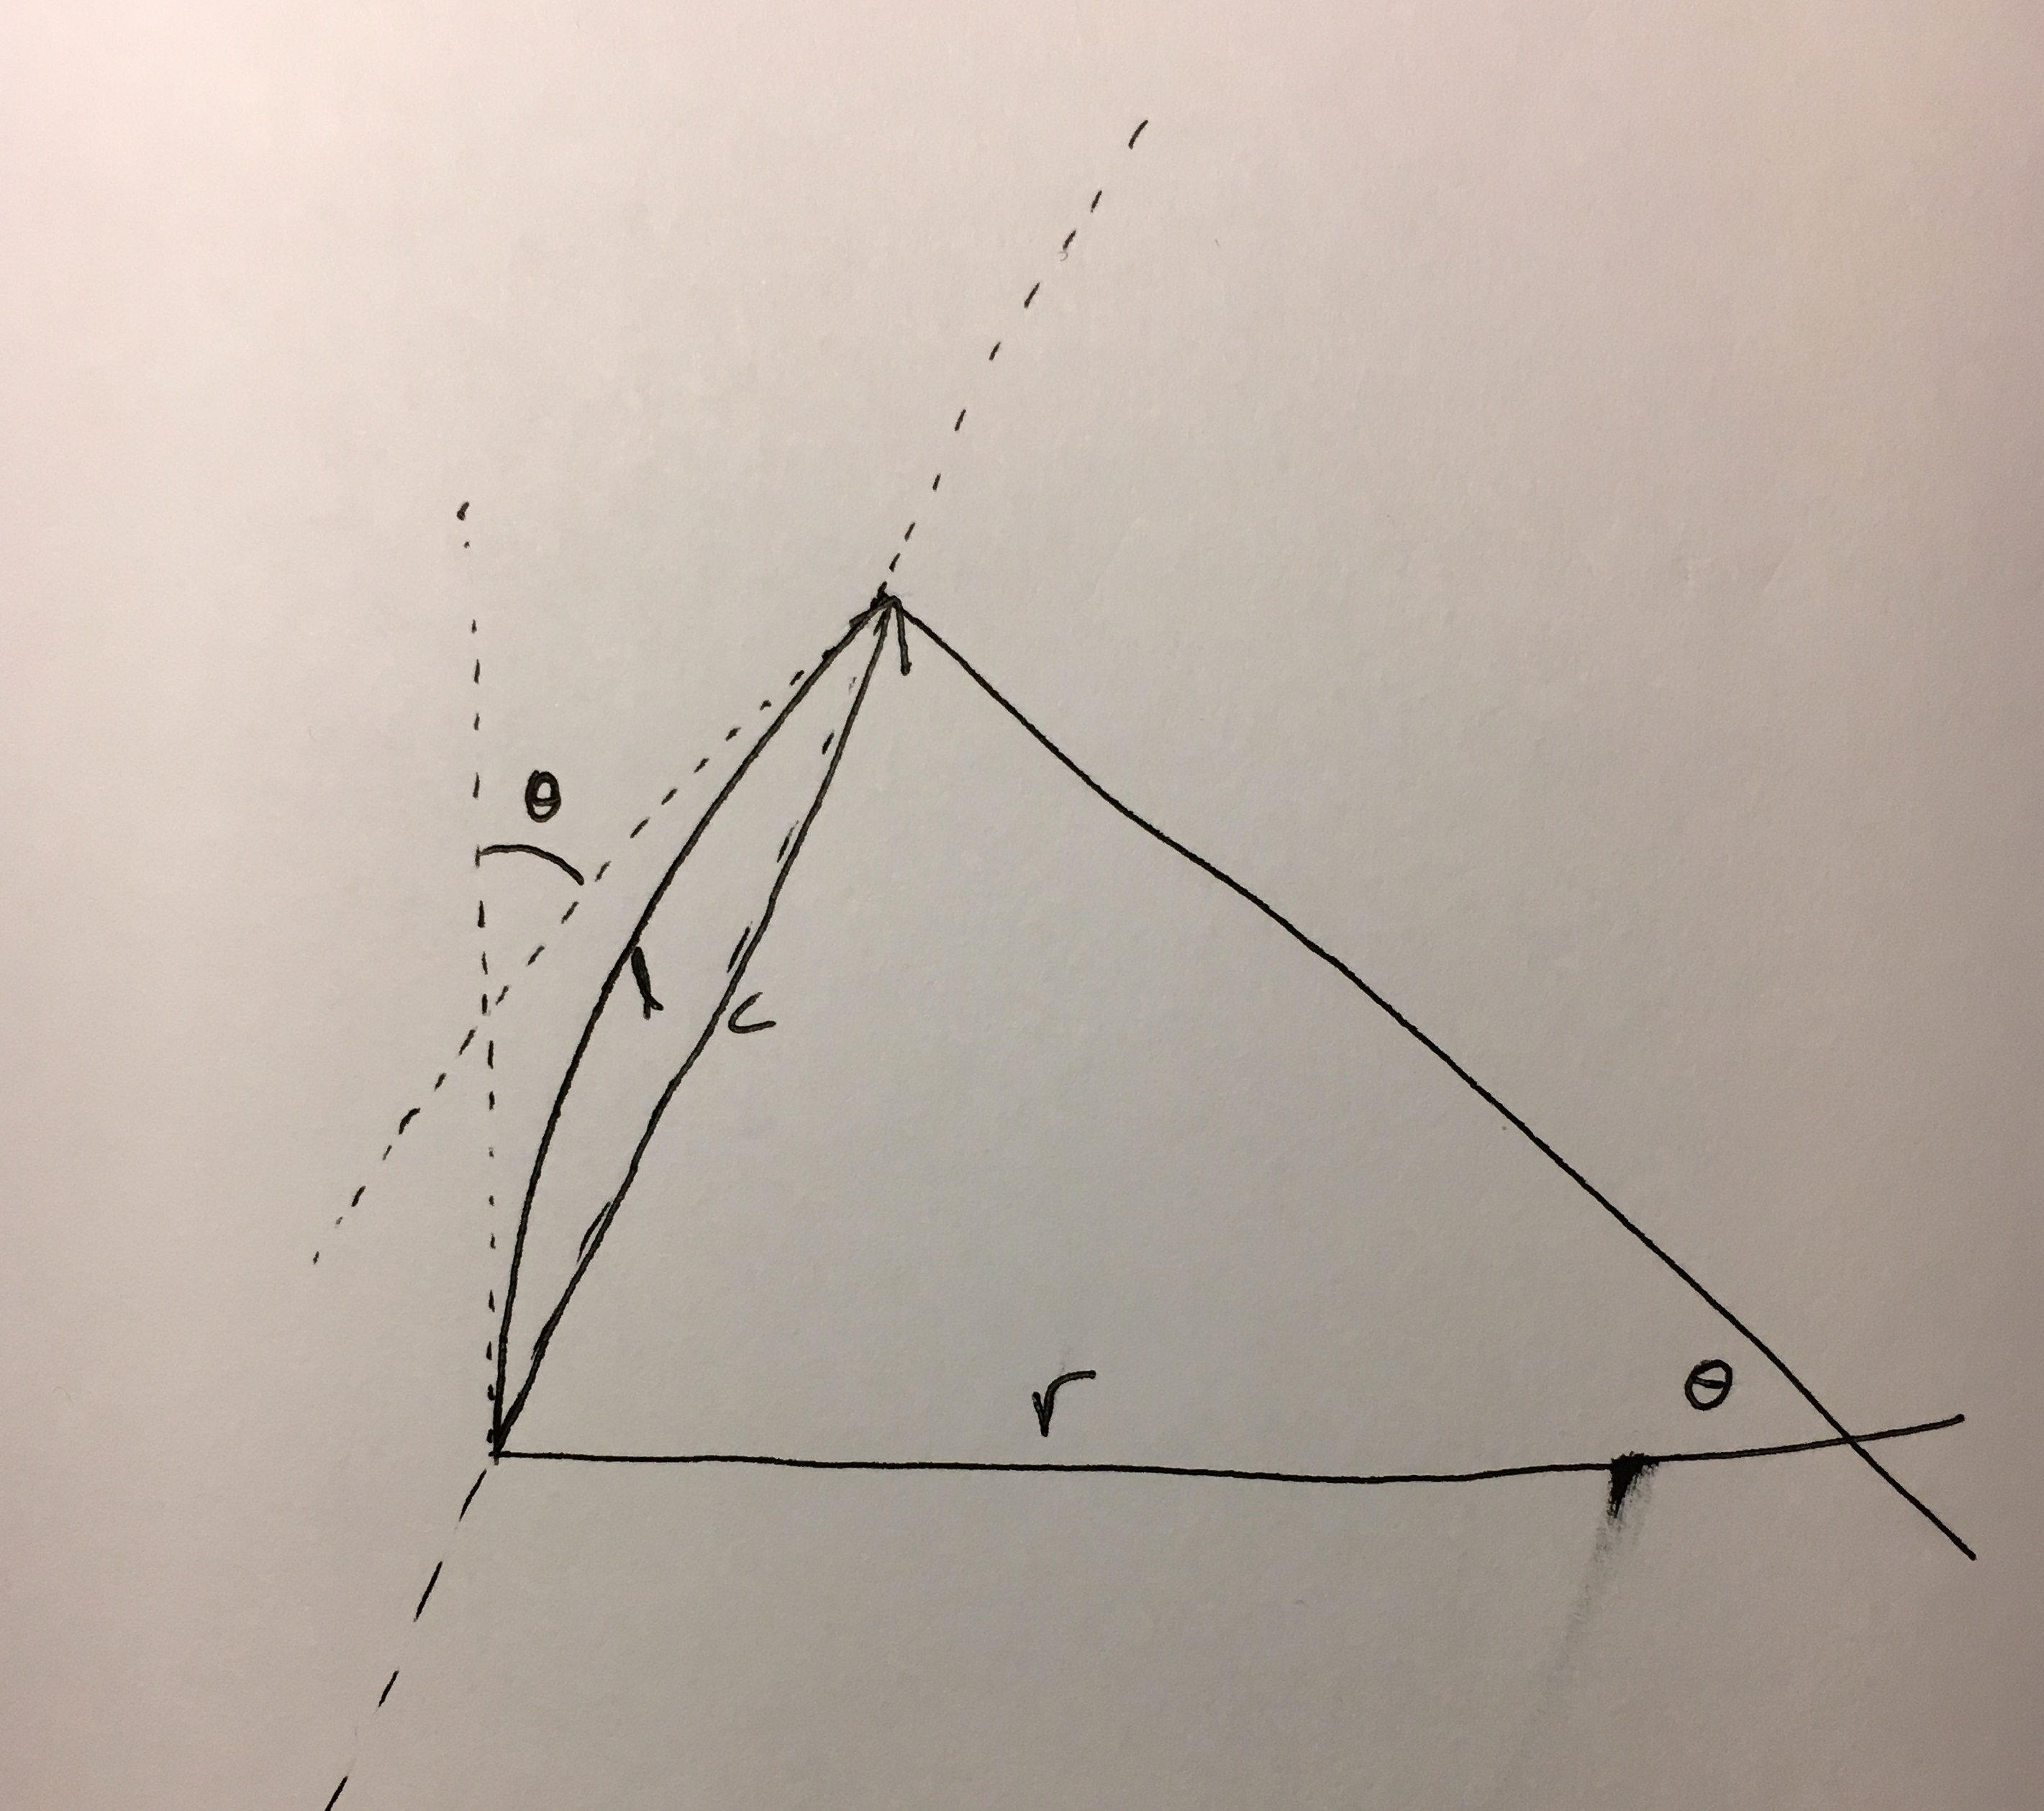
\includegraphics[width=.6\textwidth]{02/images/twist.jpg}
    \caption{Caption}
    \label{fig:twist}
\end{figure}
\end{document}